\section{Scalar field on Schwarszchild spacetime}
\subsection{Multipole moment decomposition}
\subsection{Hyperboloidal compactification}
Tortoise coordinates and wave equation
Wave equation in this form
Boundary conditions
\subsection{Initial conditions}
\subsection{final results}


\begin{figure}
  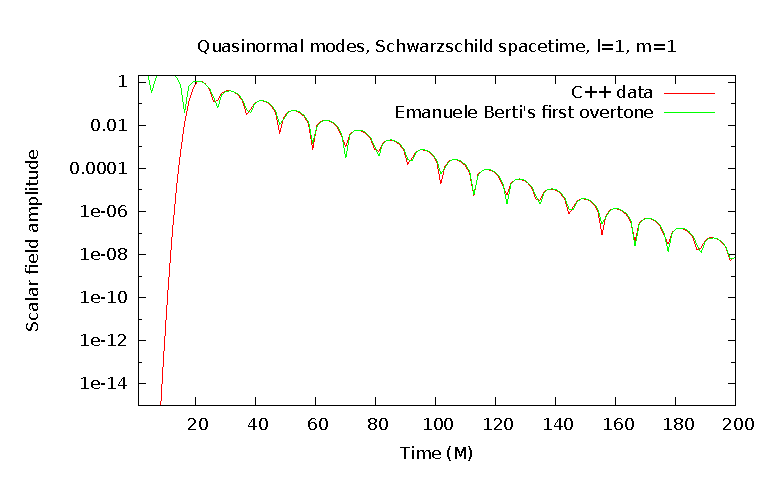
\includegraphics{l1m1qnm}
  \caption{Quasinormal mode for l=1,m=1}
  \end{figure}

\begin{figure}
  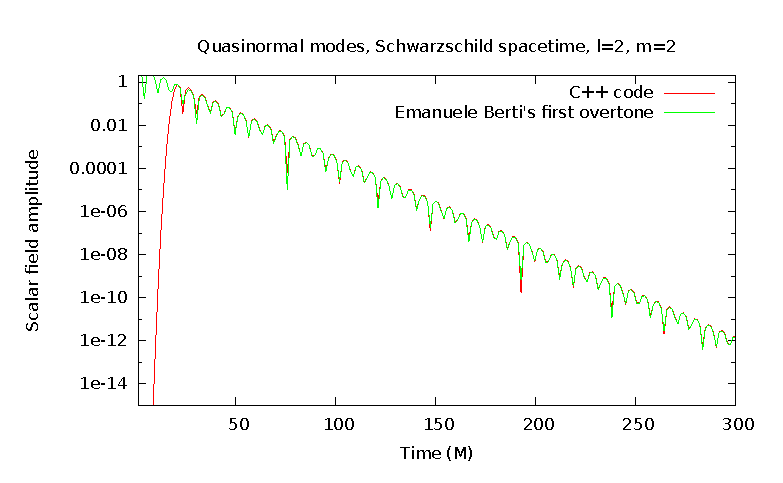
\includegraphics{l2m2qnm}
  \caption{Quasinormal mode for l=2, m=2}
\end{figure}

\begin{figure}
  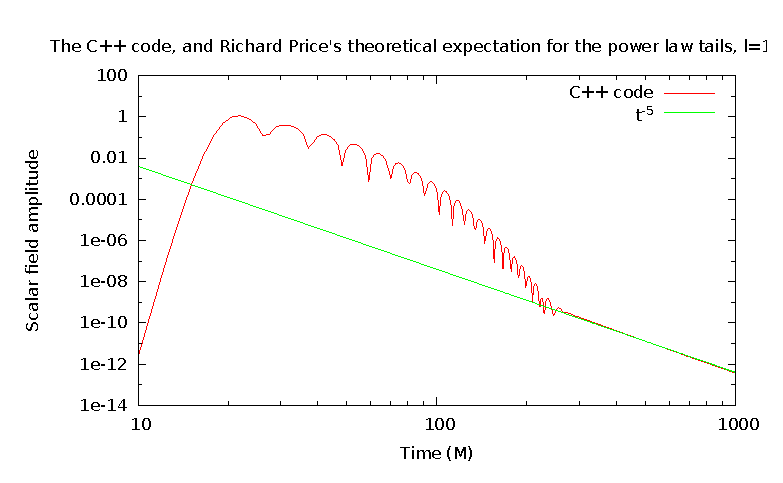
\includegraphics{l1m1tail2}
  \caption{Power law tail, l=1, m=1}
\end{figure}

\begin{figure}
  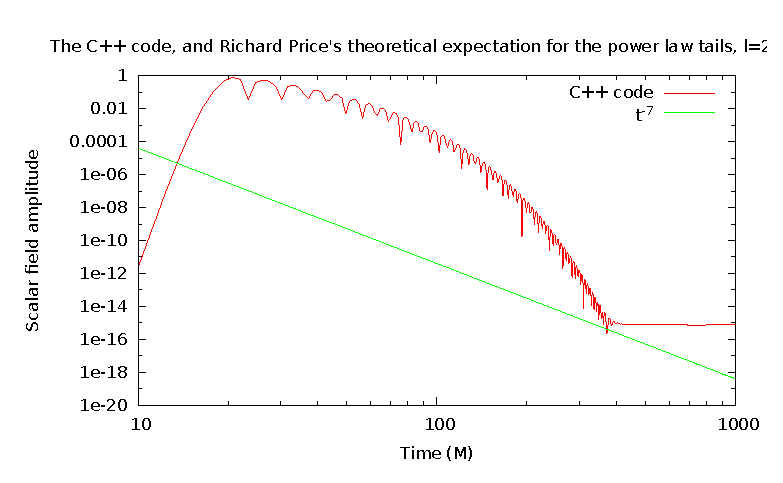
\includegraphics{l2m2tailfail2}
  \caption{Power law tail does not match expectations due to truncation error in DG method, l=2, m=2}
\end{figure}

\begin{figure}
  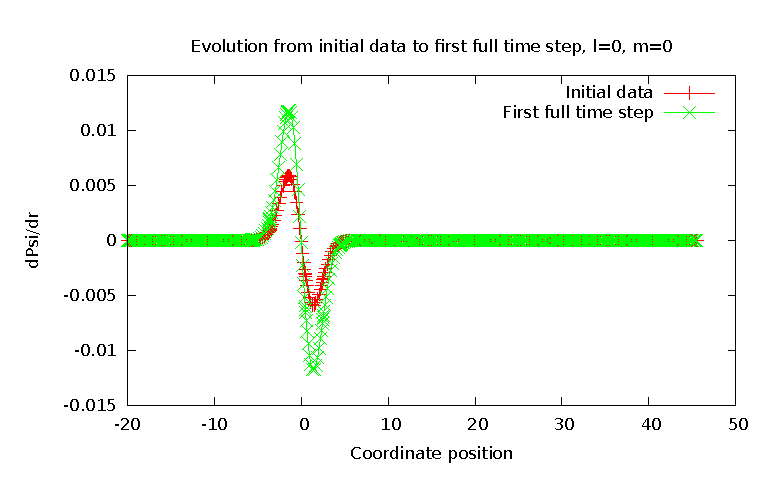
\includegraphics{phi1dl0}
  \caption{Scalar field spatial slice initial condition and first full timestep for l=0.}
\end{figure}

\begin{figure}
  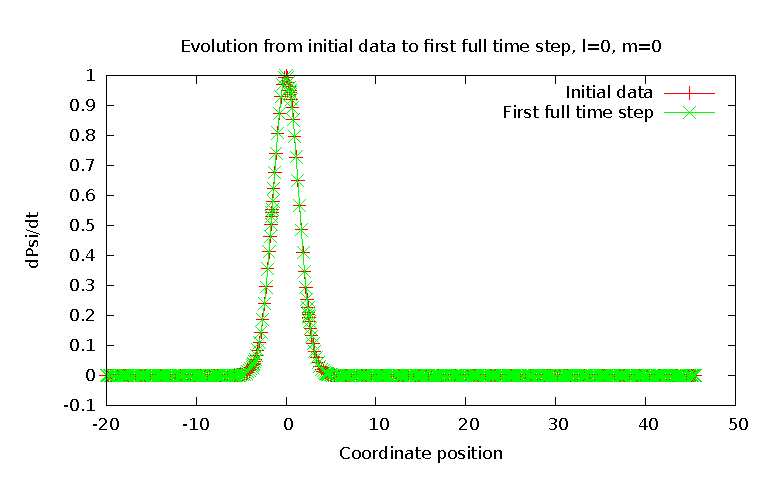
\includegraphics{rho1dl0}
  \caption{Time derivative of the scalar field spatial slice initial condition and first full timestep for l=0.}
\end{figure}

\begin{figure}
  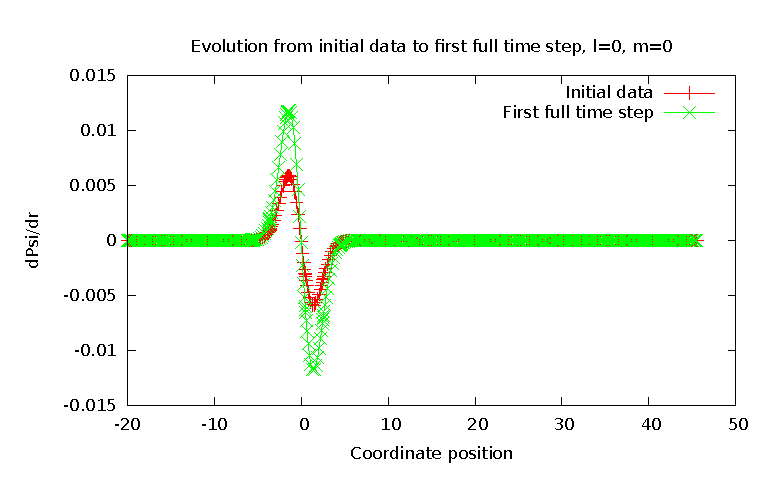
\includegraphics{phi1dl0}
  \caption{Radial derivative of the scalar field spatial slice initial condition and first full timestep for l=0.}
\end{figure}
